\section{Requirements and development}
\subsection{Ubuntu}
\begin{itemize}
	\item \textbf{CPU}: Intel X86 family;
	\item \textbf{RAM}: at least 2GB of RAM;
	\item \textbf{Disk's space}: at least 1GB.
\end{itemize}	

\subsection{Windows}
\begin{itemize}
	\item \textbf{CPU}: Intel X86 family;
	\item \textbf{Operating system}: Windows 7 or superior, 32-bit or 64-bit versions;
	\item \textbf{RAM}: at least 2GB of RAM;
	\item \textbf{Disk's space}: at least 1GB.
\end{itemize}

\subsection{MacOS}
\begin{itemize}
	\item \textbf{Mac Model}: all the models sold from 2011 onwards;
	\item \textbf{Operating system}: OS X 10.10 Yosemite;
	\item \textbf{RAM}: at least 2GB of RAM;
	\item \textbf{Disk's space}: at least 1GB.
\end{itemize}

\subsection{Development}
The product has been entirely developed using Visual Studio Code v.1.20+. A beautifier file and a dedicated workspace has been created to make the code always readable and formatted for all the developers.
To have a better look and feel sensation with the code, you can install the following extensions:
\begin{itemize}
	\item ESLint
	\item Sass Lint
	\item SCSS IntelliSense
	\item solidity
\end{itemize}
Install an extension is very simple, all you need to do is to click on the \emph{extensions} button, located in the vertical bar at the left of the screen, then type the name of the desired extension in the search bar, and click on the \textbf{Install} button once you have find it.
\begin{figure}[H]
	\centering
	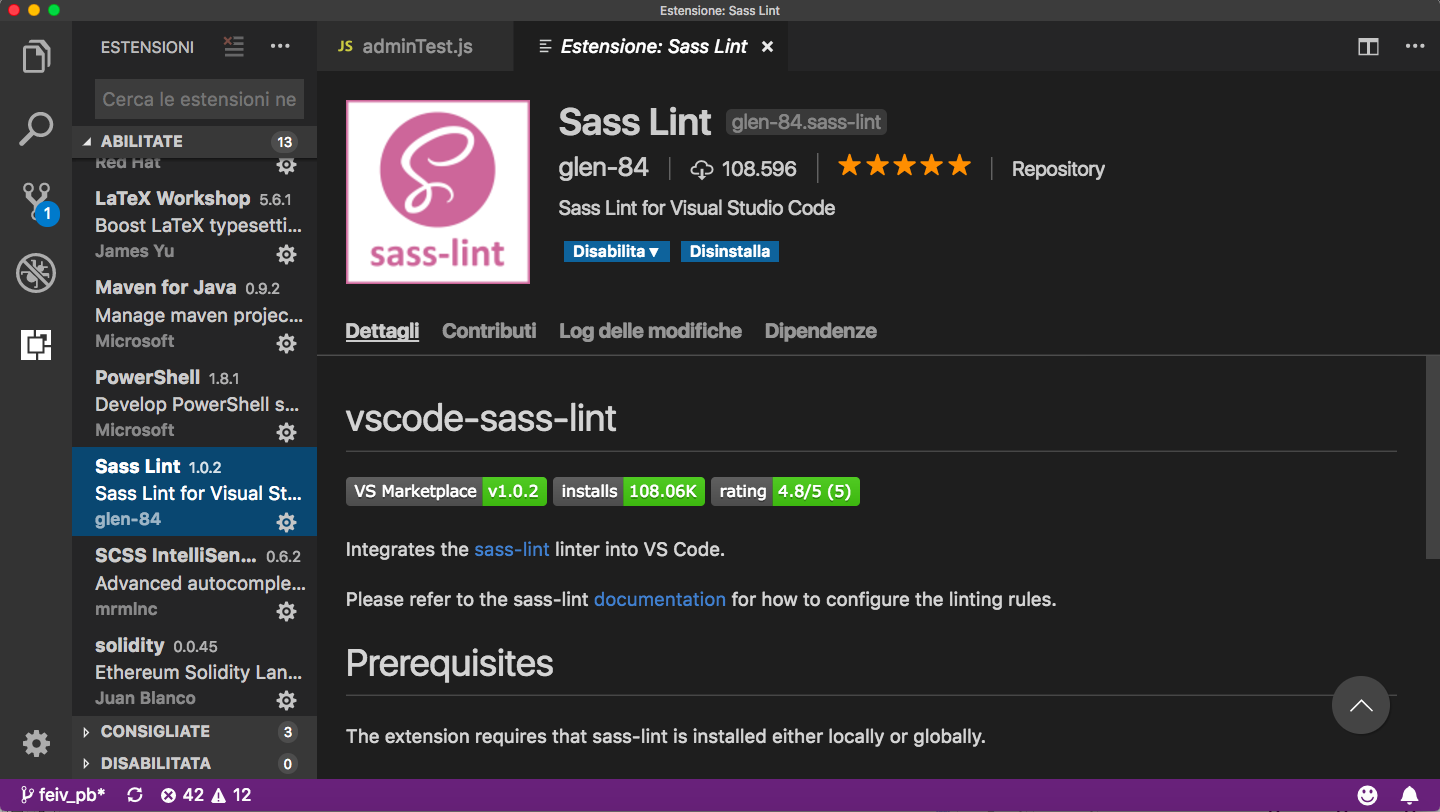
\includegraphics[width=0.42\textwidth]{img/extensions.png}
	\caption{Visual Studio Code extensions}
	\label{fig:extensions}
\end{figure}
